\section{Appendices}

\appendix

\section{Calculations for expected number of death}

Assuming that BC allocates all 246,700 doses to front-line workers, we can estimate the expected number of deaths due to VIPIT, $E(death)_{VIPIT}$, as shown below. To err on the side of caution, we assume that each dose of the vaccine is independently associated with the risk for VIPIT and that the risk of VIPIT is uniform across all age groups. We also assume that there is enough uptake that BC is able to administer all these doses.

$$
E(\text{death})_{\text{VIPIT}}  = d \times P(\text{VIPIT}|\text{vaccine}) \times P(\text{death}|\text{VIPIT})
$$

where d is the number of doses administered,  $P(\text{VIPIT}|\text{vaccine})$ is the risk of VIPIT after receiving each dose, and $P(\text{death}|\text{VIPIT})$ is the case fatality for VIPIT. 

According to the most recent data from UK and EU submitted to EudraVigilance (as of April 4th, 2021):

$$
\begin{aligned}
E(\text{death})_{\text{VIPIT}} & = d \times \frac{1}{153,000} \times \frac{21}{100} \\
& = 246,700 \times \frac{2.1}{1,530,000} \\
& \approx 0.338
\end{aligned}
$$

Considering both doses of the vaccine, we will have:

$$
\begin{aligned}
E(\text{death})_{\text{VIPIT}} & = d \times \frac{1}{153,000} \times \frac{21}{100} \\
& = 2 \times 246,700 \times \frac{2.1}{1,530,000} \\
& \approx 0.677
\end{aligned}
$$

NACI had based its analysis on the more pessimistic estimates of a chance of 1 in 100,000 for VIPIT, and a mortality probability of 40\%. In this worst-case scenario analysis, the expected number of deaths in BC would be 1:

$$
\begin{aligned}
E(\text{death})_{\text{VIPIT-Worst Case}} & = d \times \frac{1}{100,000} \times \frac{40}{100} \\
& = 246,700 \times \frac{4}{1,000,000} \\
& \approx 1
\end{aligned}
$$

Considering both doses of the vaccine, the expected number of deaths in BC would be 2. 

\section{Sensitivity Analysis}

Figure A1 summarizes projected COVID-19 case counts, hospitalizations, and deaths, for a wider range of values for $R_0$ and the effectiveness of the vaccine against transmission, $v_e$. Sensitivity analysis on vaccine effectiveness against severe disease, $v_p$, lead to similar results and conclusions with a slight variation in number of outcomes. As $v_p$ increased, both the overall number of deaths and the number of deaths prevented decreased.

\begin{figure}[htb]
\begin{center}
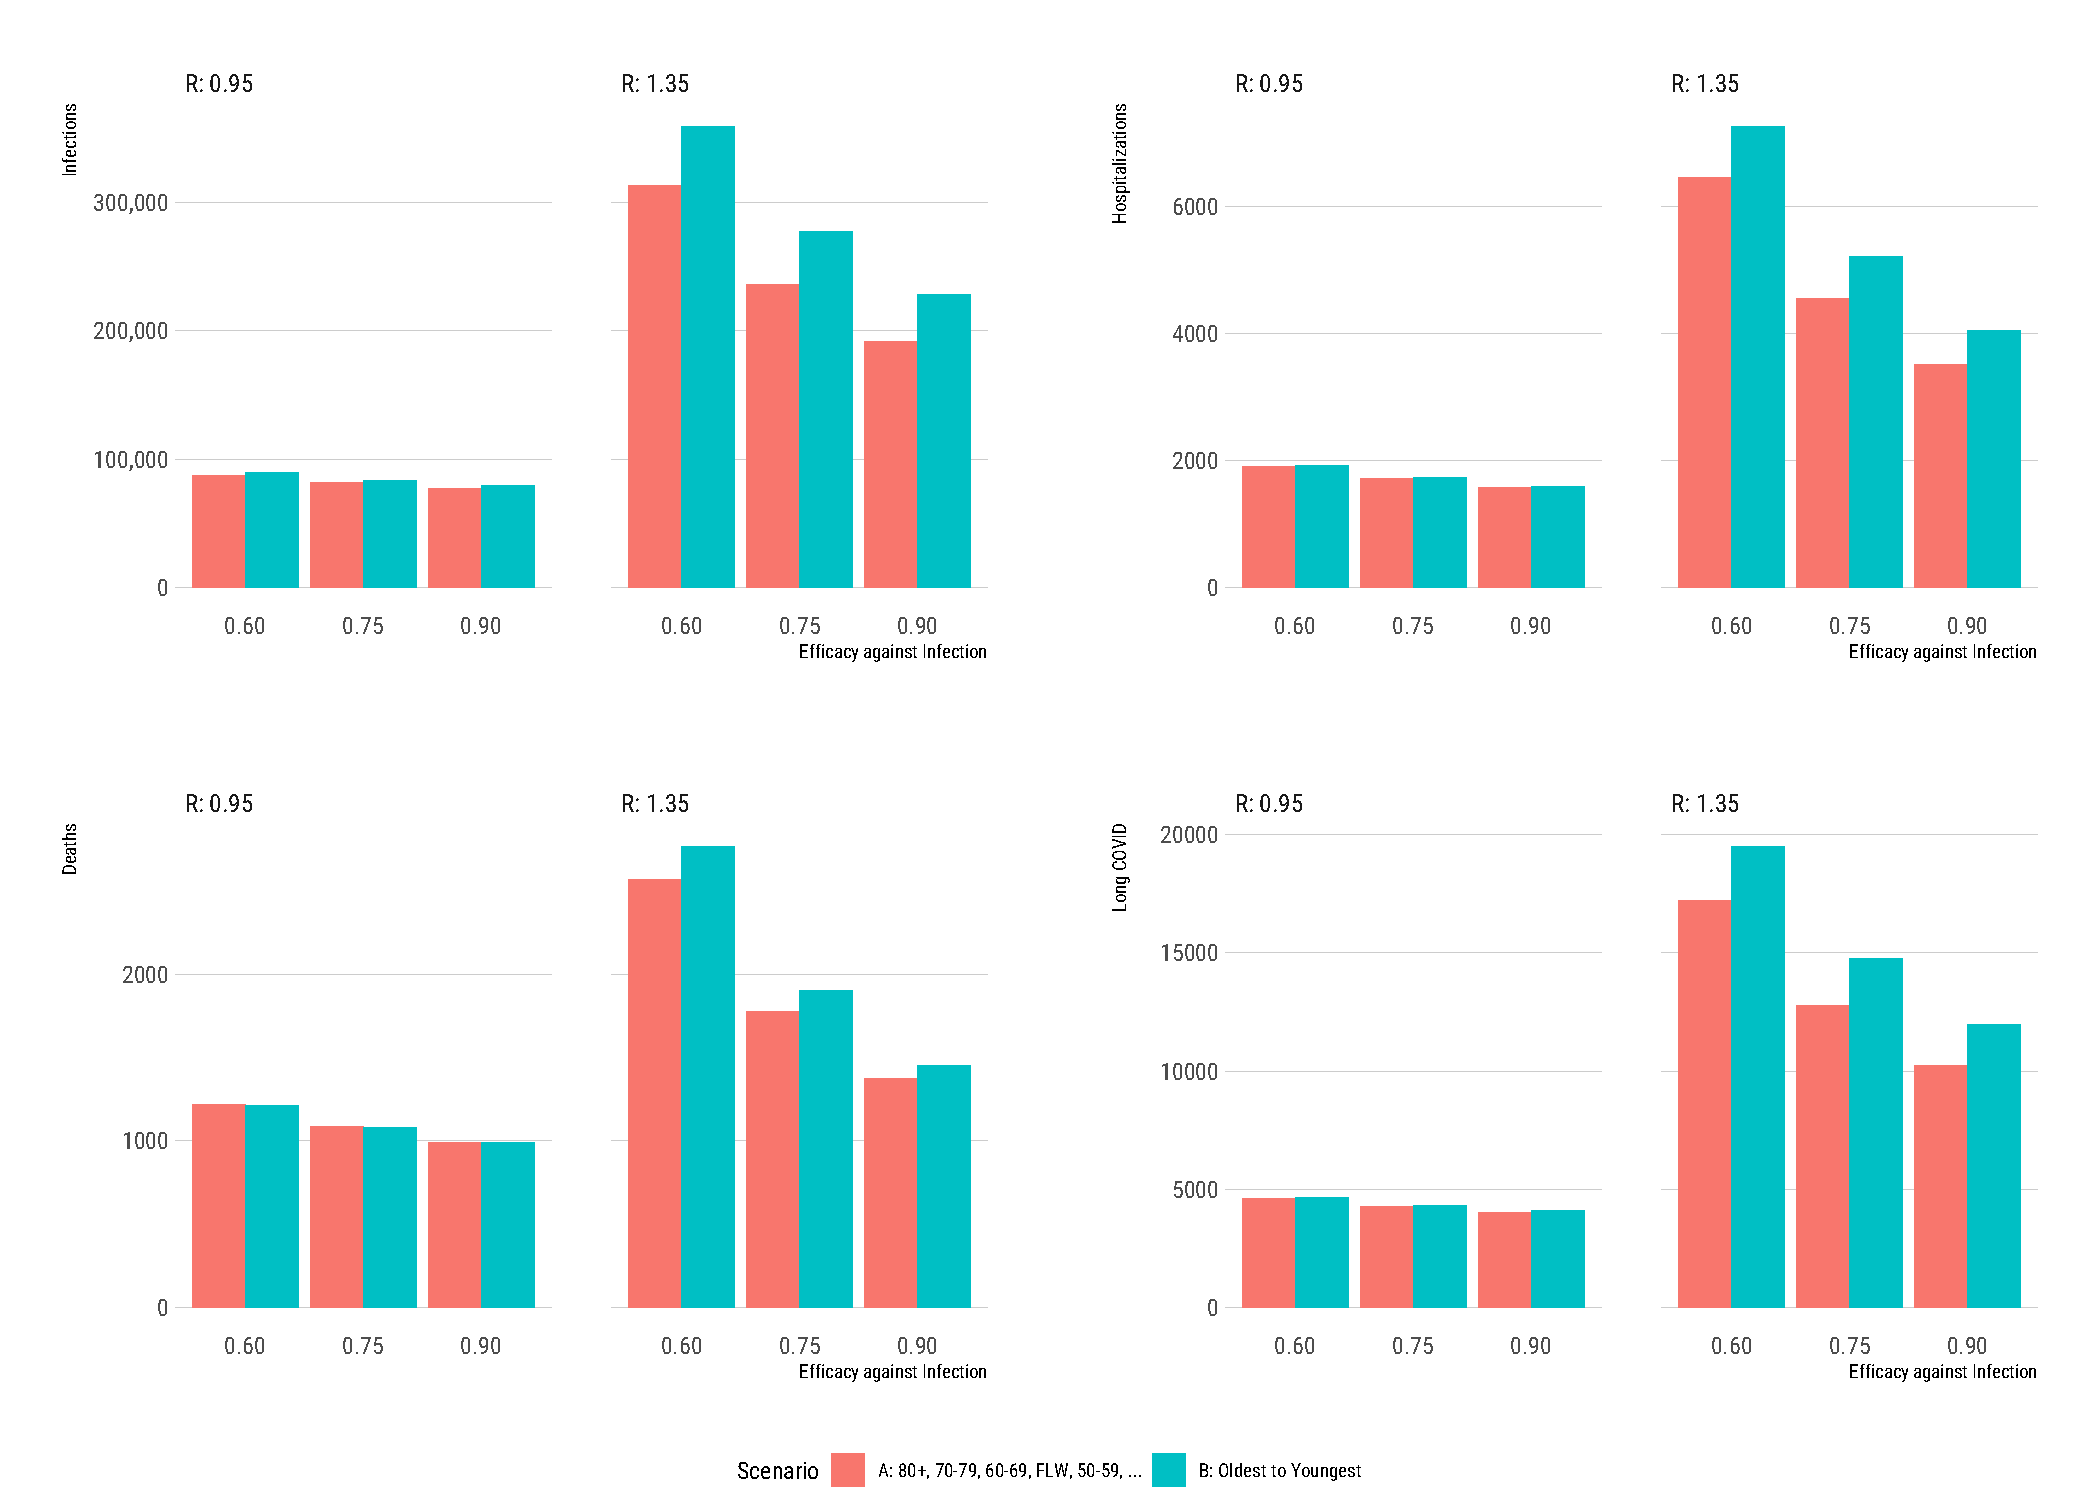
\includegraphics[width=6in]{"../figures/fig-barplots.pdf"}
\caption{COVID-19 outcomes under different vaccination scenarios for different age groups and front-line workers (FLW)}
\end{center}
\end{figure}


